\section{Visualization task}
\textbf{Using the same volume dataset: a. Choosing two different presets for the transfer function, produce different changes into the transfer function to obtain different results.}\\

Using the colume rendering module, we can use different presets. Those presets have different transfer functions that produce very different outputs. For this exercise we have selected the following presets:
\begin{itemize}
    \item CT-Bones
    \item CT-Lungs
\end{itemize}

\subsection{CT-AAA}
This preset is for visualizing the thoracic bones. We modified slightly the transfer function to  make it look as this:

\begin{figure}[H]
    \centering
    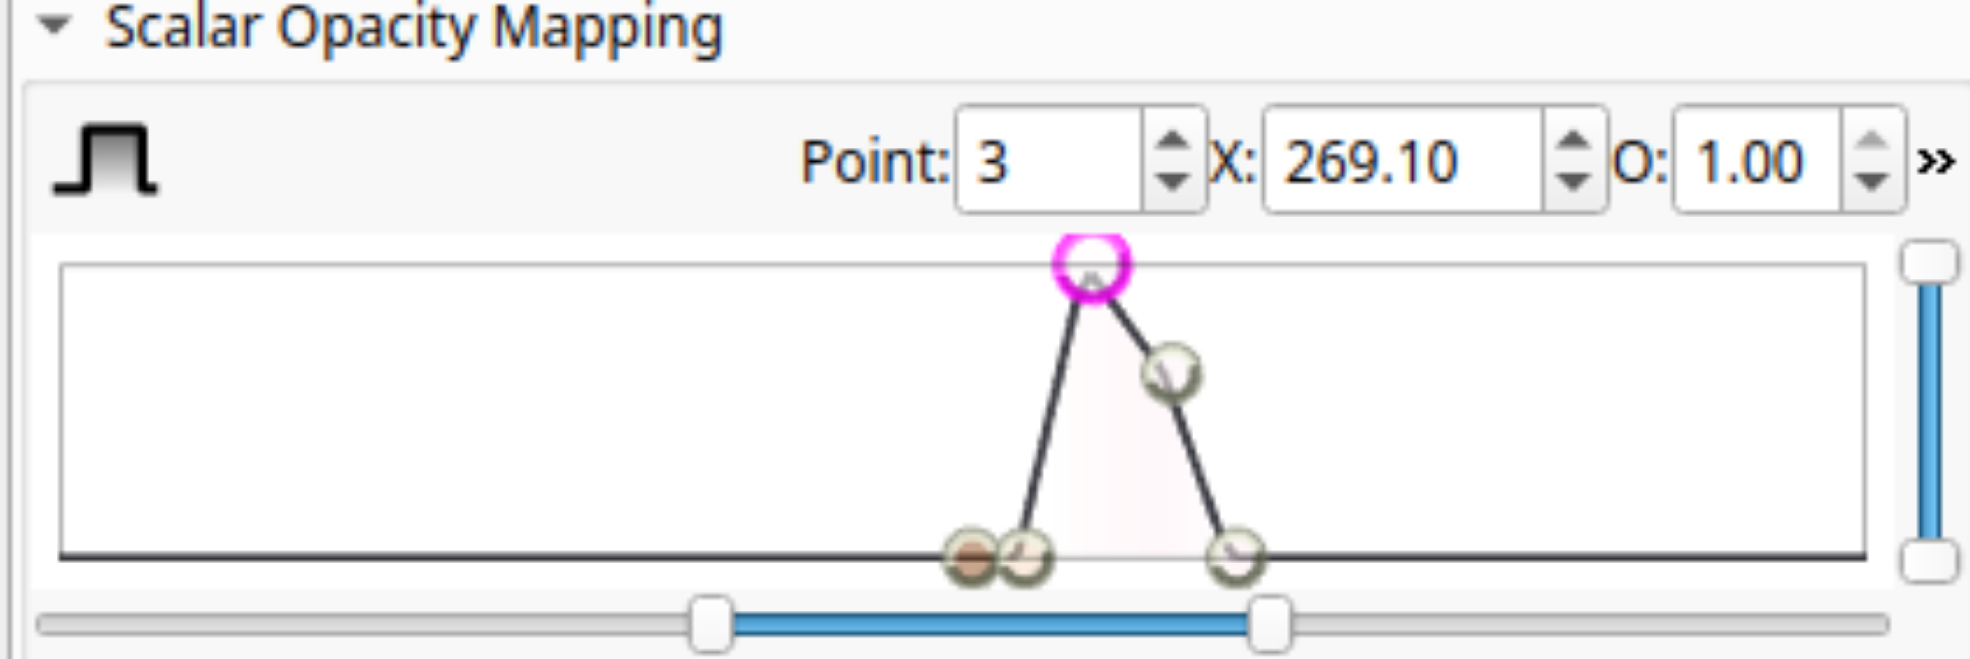
\includegraphics[width=0.7\textwidth]{img/ex21.png}
    \caption{Visualization of the thoracic bones using the CT-Bones preset with a modified transfer function.}
    \label{fig:ct_bones}
\end{figure}

Which produced the following output:
\begin{figure}[H]
    \centering
    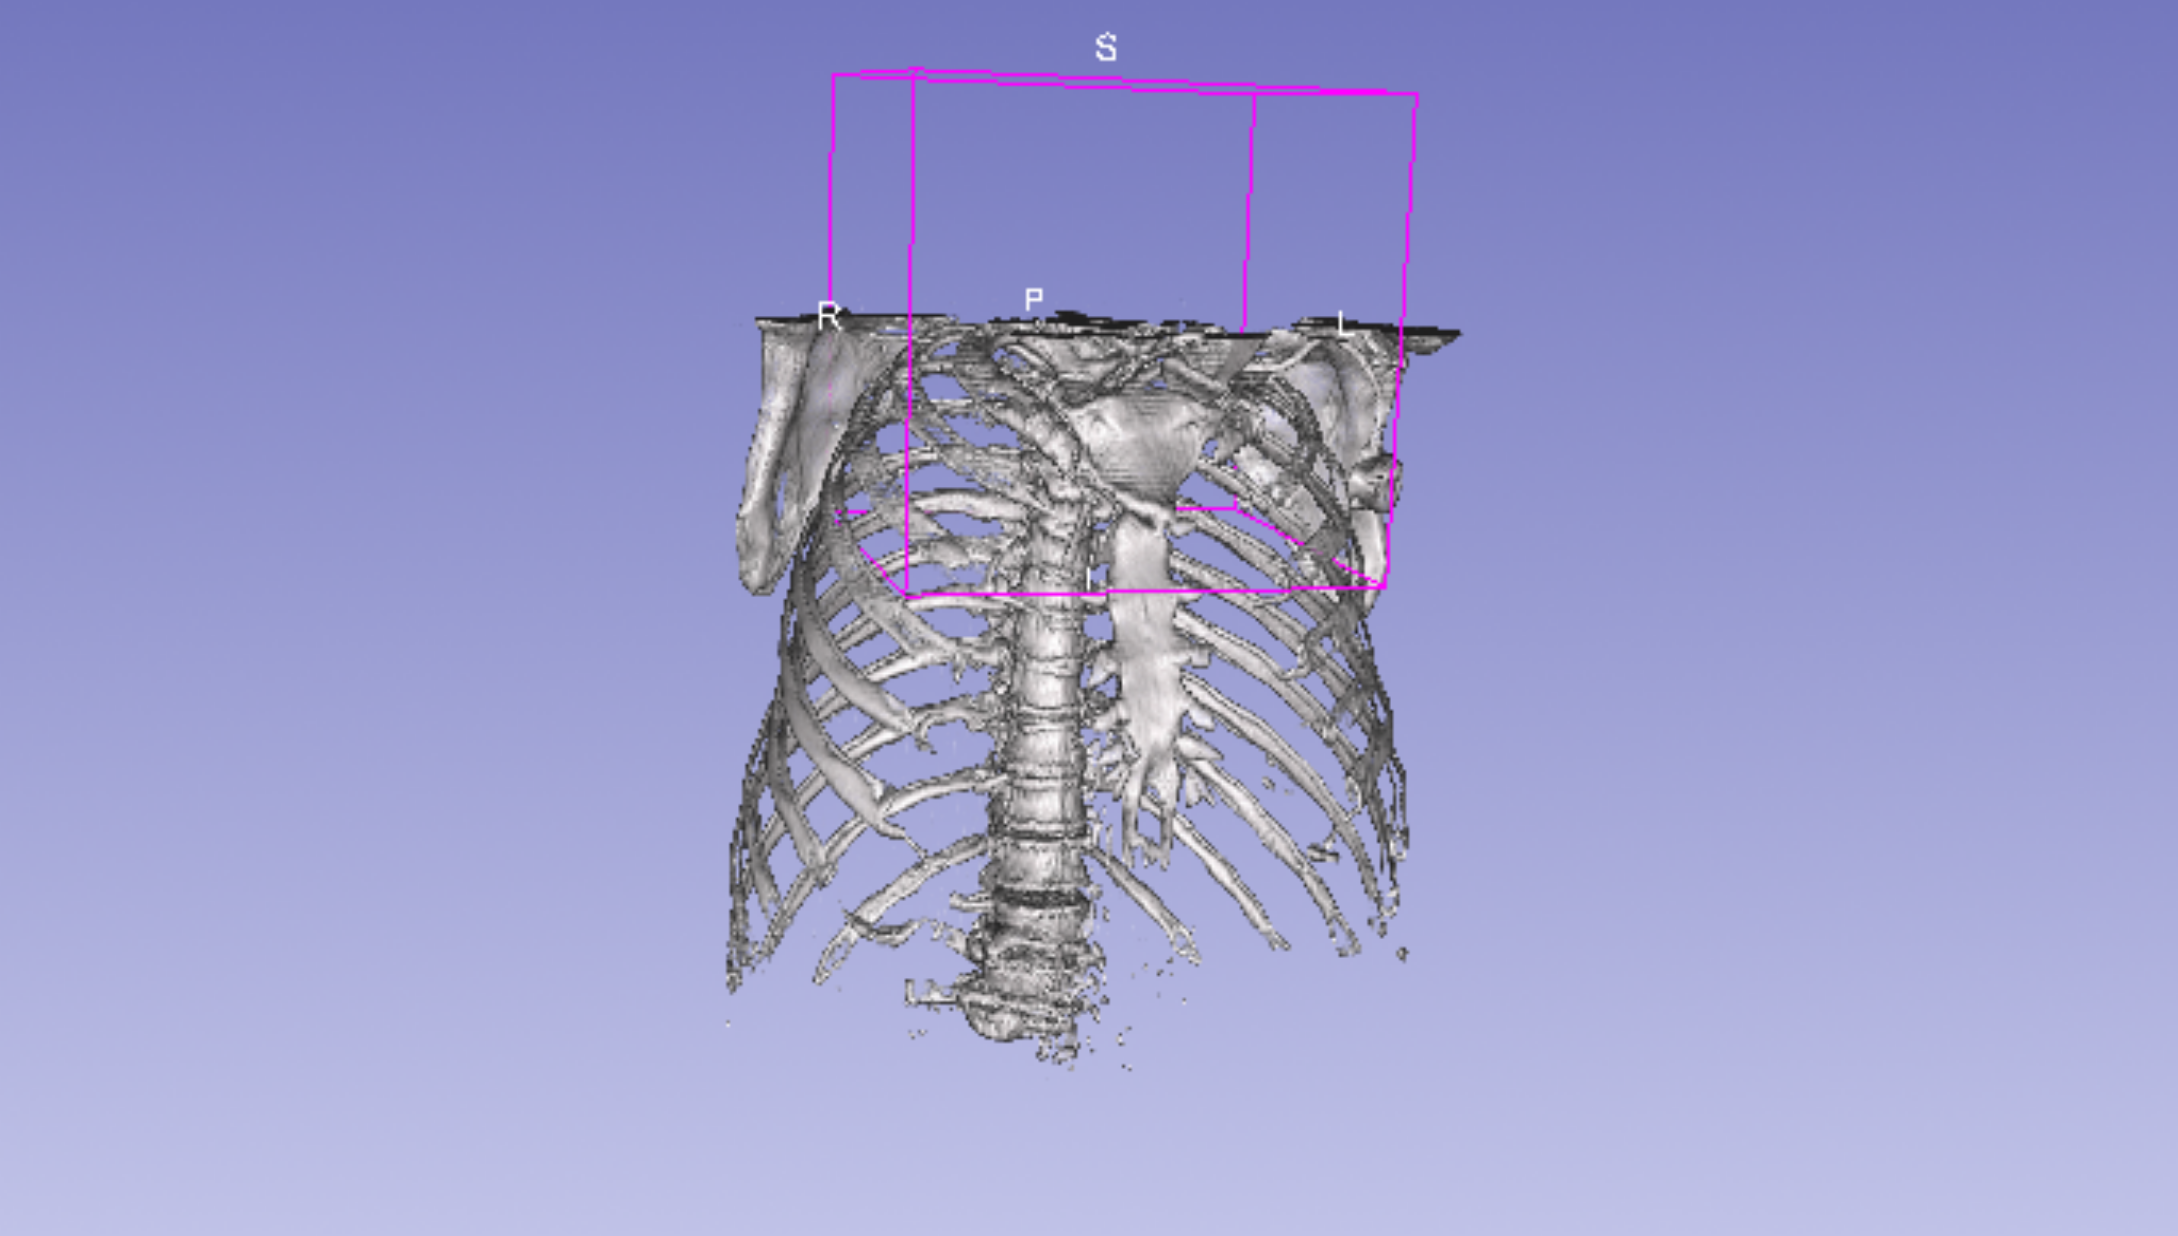
\includegraphics[width=0.6\textwidth]{img/ex22.png}
    \caption{Output of the CT-Bones preset with a modified transfer function.}
    \label{fig:ct_bones_output}
\end{figure}

\subsection{CT-Lungs}
For the lungs preset, we leaved it as it was, because it was selecting correctly the voxels corresponding to the lungs.

\subsubsection*{Transfer Funciton:}
\begin{figure}[H]
    \centering
    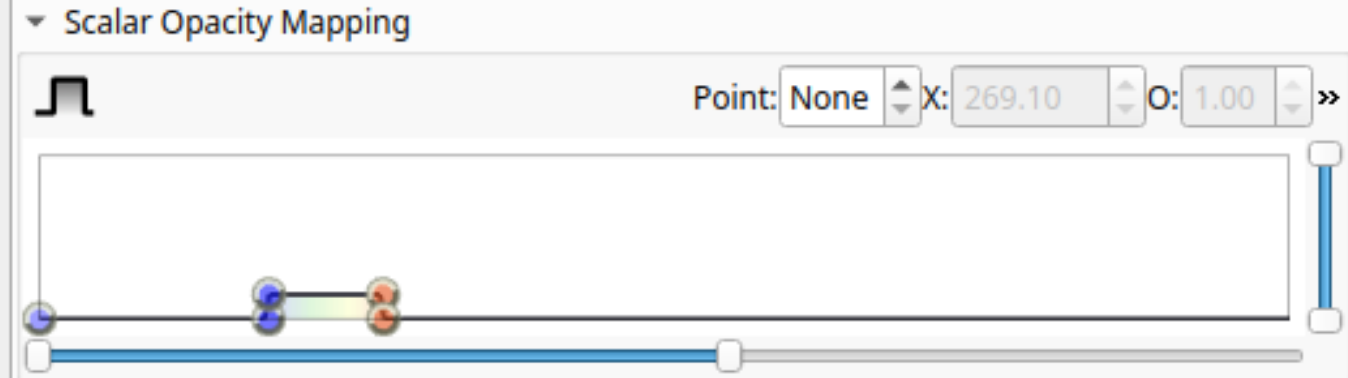
\includegraphics[width=0.5\textwidth]{img/ex24.png}
    \caption{Transfer function of the CT-Lungs preset.}
    \label{fig:ct_lungs_tf}
\end{figure}


\subsubsection*{Output:}
\begin{figure}[H]
    \centering
    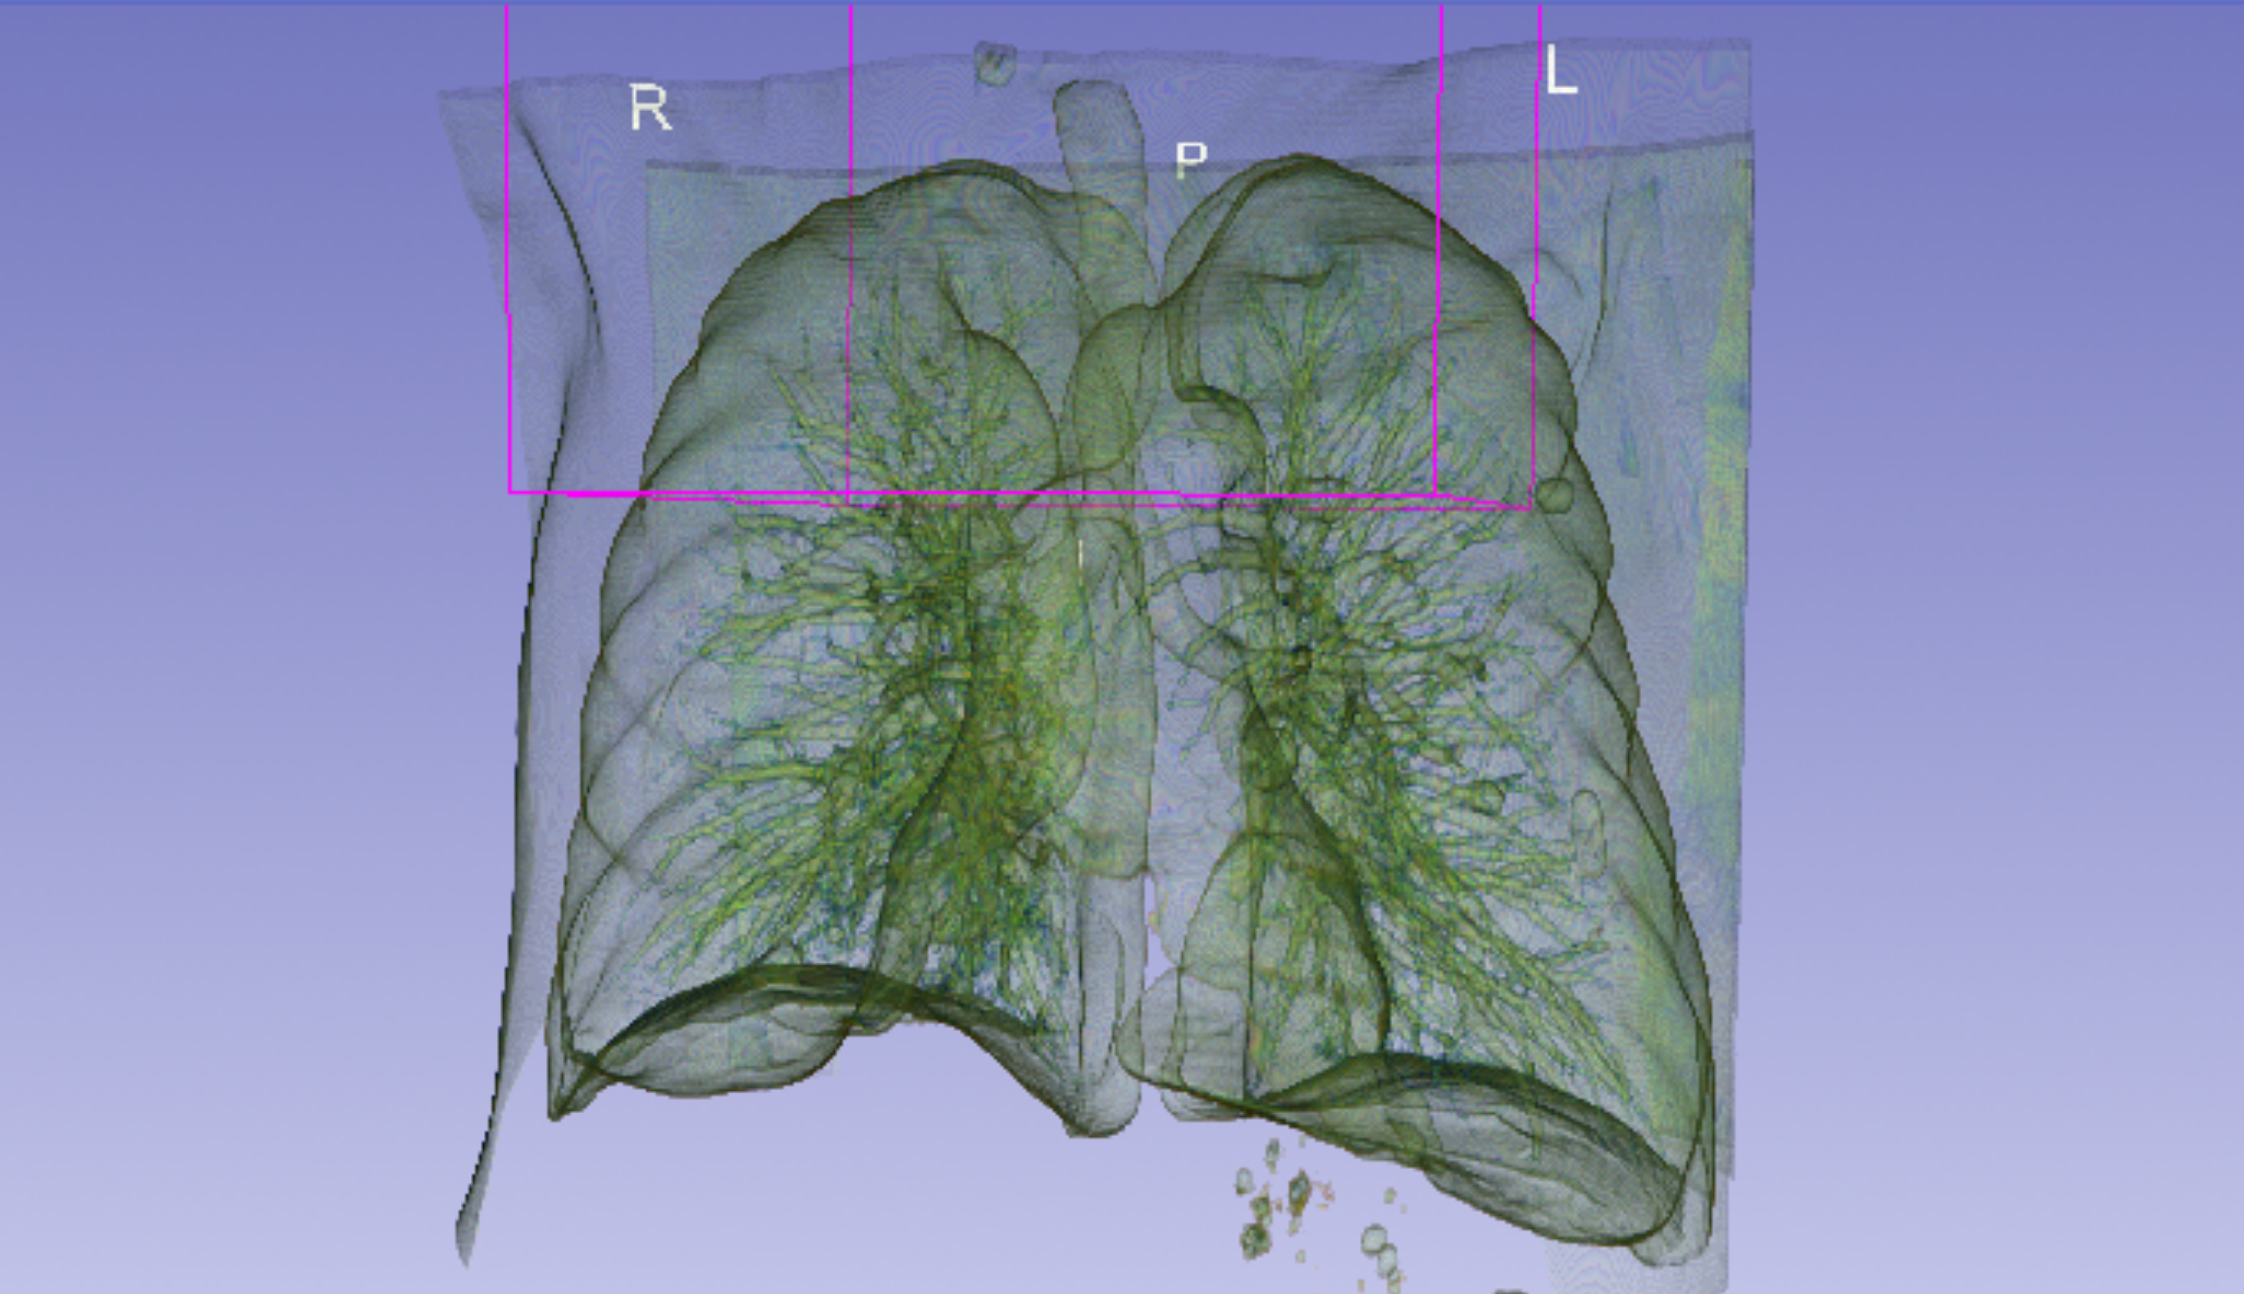
\includegraphics[width=0.6\textwidth]{img/ex23.png}
    \caption{Output of the CT-Lungs preset.}
    \label{fig:ct_lungs_output}
\end{figure}